\documentclass[10pt]{exam}
\usepackage[phy]{template-for-exam}
\usepackage{tikz}
\usepackage[top=0.2in, bottom=0.5in, left=0.5in, right=0.4in]{geometry}


\begin{document}
\pagestyle{empty}

\def\mytitle{Ch 8 Test: Momentum}

\newcommand{\topmatter} {

  \section*{Equations}

  \begin{align*}
    p &\equiv mv &
    J &\equiv F\Delta t &
    \Sigma F &= \frac{\Delta p}{\Delta t} &
    \Sigma p &= \Sigma p ' &
    v_A + v_A' &= v_B + v_B' &
    x_{CM} &= \frac{\Sigma m_i x_i}{\Sigma m_i}
  \end{align*}

  \vfill
  
  \section*{Instructions}

  \begin{enumerate}
    \item Put your name on this page and \textbf{bubble in your 8-digit Student ID number} (400....).
    \item Tear off this front page.
    \item Put your name on the top of the rest of the packet.
    \item The problems are on the first two pages, the next page contains the bonus problems, and the next page contains all of the multiple choice.
    \item You may write on anything, but I'm only grading this page and the first three pages of the rest of the packet.
    \item The equations are provided above.
  \end{enumerate}

}

\newcommand{\drawscantron}[2]{
  \begin{tikzpicture}
    \node[anchor=south west] at (0,0) {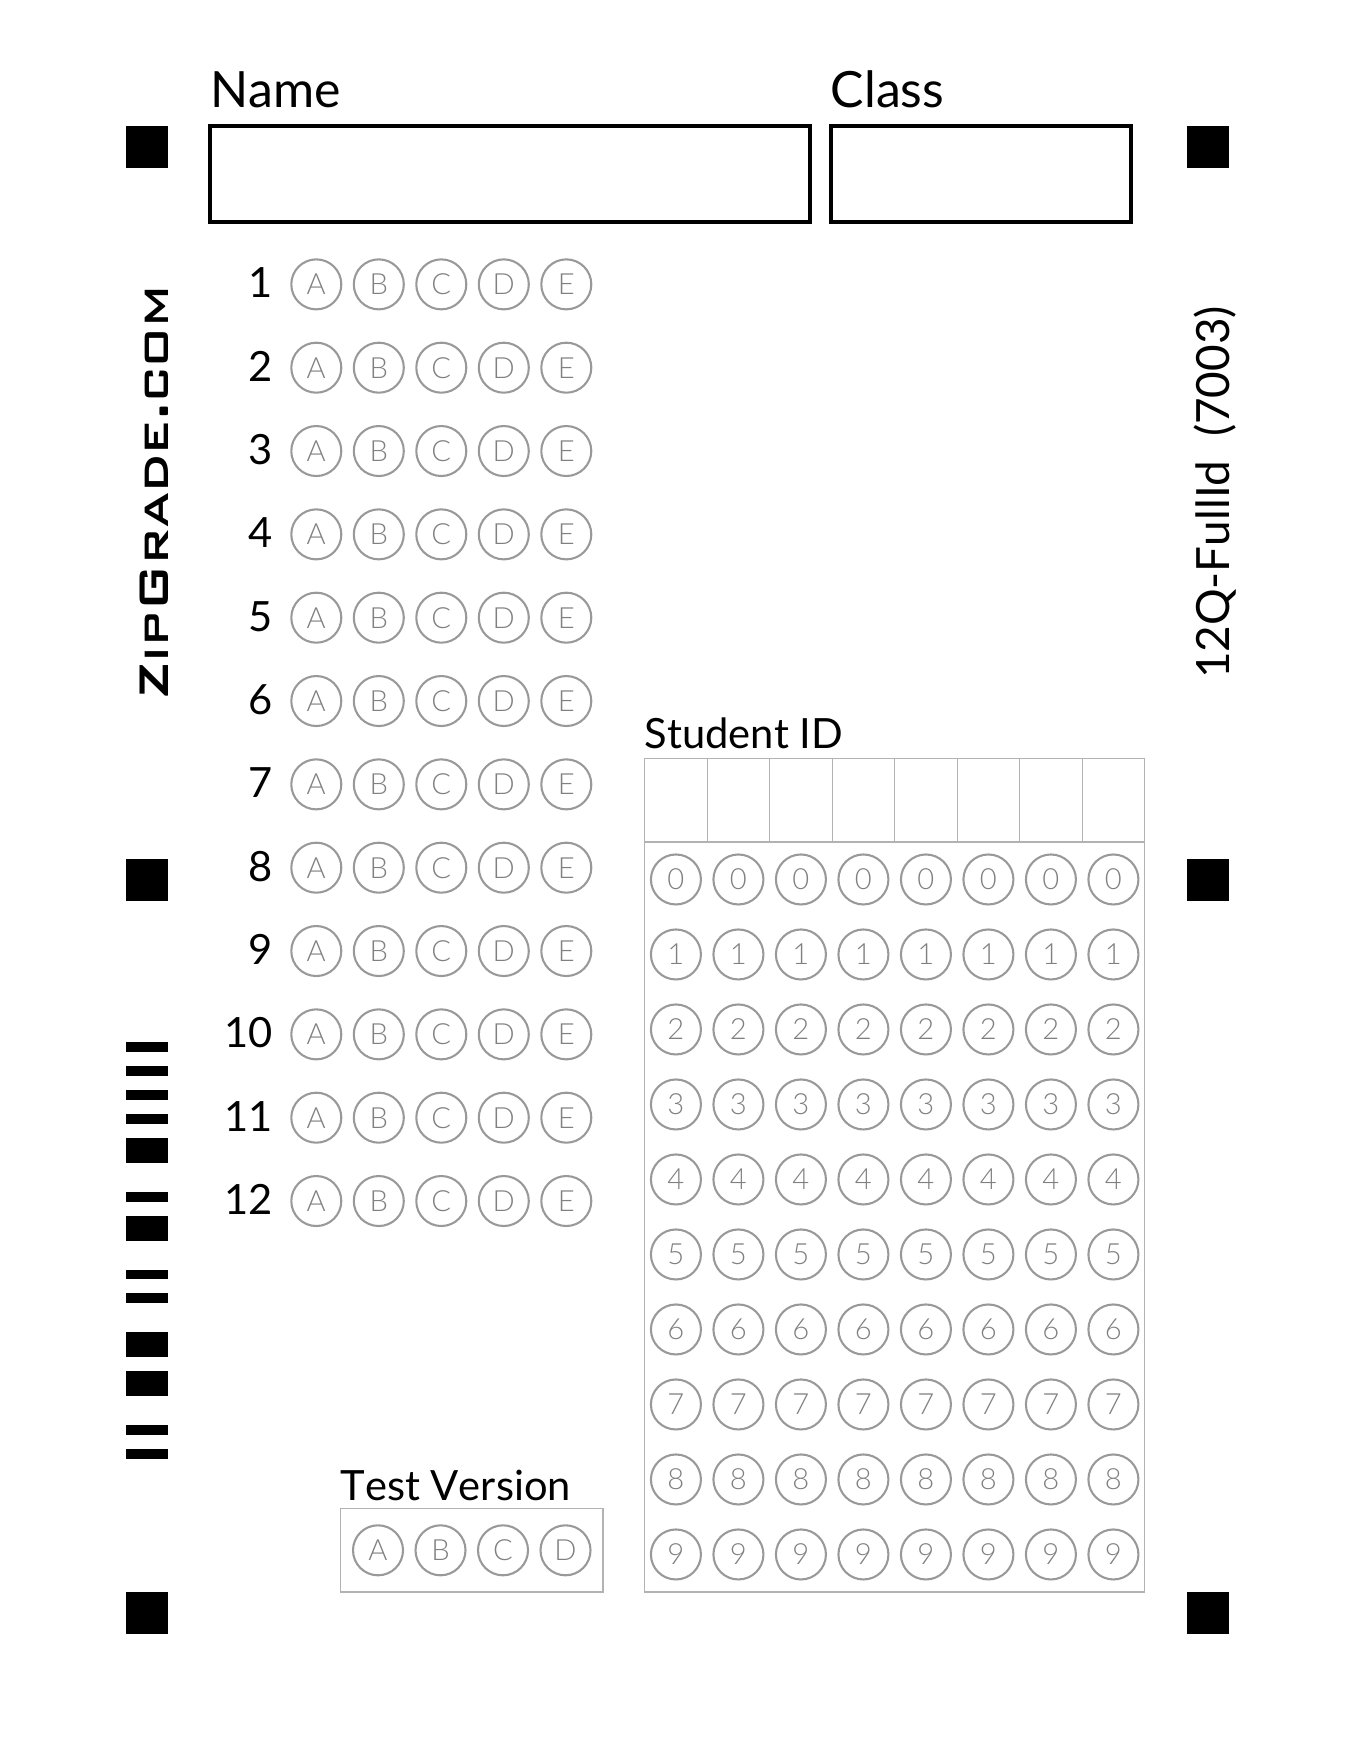
\includegraphics[height=5in]{12Q.png}};
    \fill (#1,#2) circle (0.2);
    \node[anchor=west] at (-8.6,12) {\LARGE \bf \sc \mytitle};
  \end{tikzpicture}
}



  \drawscantron{2.85}{1.65}
  \topmatter

\pagebreak

  \drawscantron{3.3}{1.65}
  \topmatter

\pagebreak

  \drawscantron{3.75}{1.65}
  \topmatter

\pagebreak

  \drawscantron{4.2}{1.65}
  \topmatter


\end{document}